% !TEX program  = xelatex

\documentclass{article}
\usepackage{ctex}
\usepackage{xeCJK}
\usepackage[ruled,vlined,linesnumbered]{algorithm2e}
\usepackage{algpseudocode}
\usepackage{amsmath}
\usepackage{amsthm}
\usepackage{graphicx}
\usepackage{subfigure}
\usepackage{float}
\usepackage{amsmath }
\usepackage{amsfonts }
\usepackage{pdfpages}
\usepackage{epsfig}
\usepackage{graphicx}
\usepackage{arydshln}
\usepackage{verbatim}
\usepackage{subfigure}
\usepackage{enumerate}
\usepackage{rotating}
\usepackage{threeparttable}
\usepackage{caption}
\usepackage{tikz}
\usepackage{epsfig}
\usepackage{cite}
\usepackage{geometry}
\usepackage{listings}
\usepackage{xcolor}
\usepackage{fontspec}
\newfontfamily\codefont{times.ttf}
\setmainfont{times.ttf}
\newcommand{\customthmname}{}
\newenvironment{prob}[1]
{\renewcommand{\customthmname}{#1}%
	\fontfamily{ptm}\selectfont  % 设置 Times 字体
	\par\bigskip\noindent\Large{\customthmname}\normalsize\par}
{\par\bigskip}
\newtheorem{ans}{Answer}
\setCJKmainfont{SourceHanSerifCN-Regular-1.otf}
\newcommand{\textbff}[1]{\textcolor{red}{\textbf{#1}}}
\lstdefinestyle{armasm}{
	frame=tb,
	aboveskip=3mm,
	belowskip=3mm,
	showstringspaces=false,
	columns=flexible,
	framerule=1pt,
	rulecolor=\color{gray!35},
	backgroundcolor=\color{gray!5},
	basicstyle={\small\ttfamily},
	numbers=left,
	numberstyle=\tiny\color{gray},
	numbersep=5pt,
	keywordstyle=\color{blue},
	commentstyle=\color{green!50!black},
	stringstyle=\color{red!80!black},
	breaklines=true,
	breakatwhitespace=true,
	tabsize=3,
	identifierstyle=\color{black},
	emphstyle=\color{purple},
	morecomment=[l][\color{magenta}]{@},
	keywords={add, sub, mov, bx, bl, ldr, str, cmp, bne, b, lsl, mrs, adr, msr},
	emph={r0, r1, r2, r3, r4, r5, r6, r7, r8, r9, r10, r11, r12, r13, r14, r15, lr, sp, pc, x9},
}
\geometry{a4paper, top=2.4cm, bottom=2.4cm, left=3.18cm, right=3.18cm}
\usepackage[colorlinks,linkcolor=black]{hyperref}
\linespread{1.2}
\begin{document}
	\title{CS3601 操作系统 ChCore Lab 2}
	\author{王凯灵 521030910356}
	\date{2023.11.1}
	\maketitle
	\begin{prob}{练习题 1}
		完成 \texttt{kernel/mm/buddy.c} 中的 \texttt{split\_chunk}、\texttt{merge\_chunk}、\texttt{buddy\_get\_pages}、 和 \texttt{buddy\_free\_pages} 函数中的 \texttt{LAB 2 TODO 1} 部分，其中 \texttt{buddy\_get\_pages} 用于分配指定阶大小的连续物理页，\texttt{buddy\_free\_pages} 用于释放已分配的连续物理页。
	\end{prob}
	要实现这些函数首先需要看懂函数\texttt{get\_buddy\_chunk}和\texttt{init\_buddy}。阅读代码，发现实现时使用\texttt{page}结构体进行管理。在初始化时，将一定范围的物理地址按单页大小初始化到\texttt{page}中，每页对应一个结构体。初始化时，使用了需要实现的\texttt{buddy\_free\_pages}，所以首先进入这个函数。
	
	\texttt{buddy\_free\_pages}的目的是释放page并尽可能的向上合并。用于初始化时，其实会直接向上合并到最大。就结果而言，初始化结束后free list里应该只剩最大的块。\textbff{事实上}，笔者认为直接在init过程中完成大块的初始化更加自然和高效。\textbff{然而}，给出的不可改动部分指定了初始化阶段所有\texttt{page}状态为allocated。这意味着我们并不能在释放第一个page时就递归的合并所有page，而是在释放到buddy时再向前合并。每次最多只向上合并一层。这使得理解更加困难，也并不优雅。
	
	由于需要用到合并，首先实现\textbff{\texttt{merge\_chunk}}比较自然。\texttt{merge\_chunk}的实现逻辑为：使用\texttt{get\_buddy\_chunk}获取好哥们，如果哥们存在且有空，则合♂体及更新free list等，然后递归向上。这里需要注意递归中止条件是小于\texttt{BUDDY\_MAX\_ORDER}而不是等于，按头文件的定义。
	
	然后就是\textbff{\texttt{buddy\_free\_pages}}，解除allocated tag，进行merge，后更新free list即可。
	
	\textbff{\texttt{split\_chunk}}拆分思路与合并类似，order-1后将产生的buddy加入free list。我的实现还检查了大部分异常情况。
	
	最后\textbff{\texttt{buddy\_get\_pages}},寻找高于所需order的最小free块并split即可。一切要求实现的代码都贴在\textbff{附录}中。
	
	由于不知道未来上层代码会不会异常处理，我使用\texttt{BUG\_ON}宏处理了所有分配失败。
	
	\begin{prob}{练习题 2}
		完成 \texttt{kernel/mm/slab.c} 中的 \texttt{choose\_new\_current\_slab}、\texttt{alloc\_in\_slab\_impl} 和 \texttt{free\_in\_slab} 函数中的 \texttt{LAB 2 TODO 2} 部分，其中 \texttt{alloc\_in\_slab\_impl} 用于在 slab 分配器中分配指定阶大小的内存，而 \texttt{free\_in\_slab} 则用于释放上述已分配的内存。
	\end{prob}
	
	首先，笔者愚笨，并未一眼看出\textbff{\texttt{choose\_new\_current\_slab}}的作用。此函数在\\\texttt{try\_return\_slab\_to\_buddy}中调用，得知此函数用于将当前slab指向一个新slab。于是只需要从pool的partial list中有则取之即可。
	
	\textbff{\texttt{alloc\_in\_slab\_impl}}已经检查了当前Slab是否为空。TODO部分尝试取出一个slot，如果失败，则new一个，再失败就解锁并返回NUll。否则正常取出并更新状态。
	
	相比之下，\textbff{\texttt{free\_in\_slab}}的操作就很简单，只需更新状态即可。
	
	\begin{prob}{练习题 3}
		完成 \texttt{kernel/mm/kmalloc.c} 中的 \texttt{\_kmalloc} 函数中的 \texttt{LAB 2 TODO 3} 部分，在适当位置调用对应的函数，实现 \texttt{kmalloc} 功能
	\end{prob}
	只需要分别使用slab和buddy即可。其中由于本实现的buddy大小完全基于order，按理说需要更新实际大小到上层结构体中，但并没有提供接口，故忽略。
		
	至此，grade得到了30分。
		
	\begin{prob} {练习题 4}
		完成 \texttt{kernel/arch/aarch64/mm/page\_table.c} 中的 \texttt{query\_in\_pgtbl}、\texttt{map\_range\_in\_pgtbl\_common}、\texttt{unmap\_range\_in\_pgtbl} 和 \texttt{mprotect\_in\_pgtbl} 函数中的 \texttt{LAB 2 TODO 4} 部分，分别实现页表查询、映射、取消映射和修改页表权限的操作，以 4KB 页为粒度。
	\end{prob}
	首先，清楚各个参数的定义。查看vmspace结构体得知pgtbl是页表基地址，查看\texttt{get\_next\_ptp}，该函数修改传入的页表指针并返回指向类型。返回四种，无映射、无内存、指向块、指向下一级。两个错误都返回负数，直接判断小于0并将返回值返回即可。于是\textbff{\texttt{query\_in\_pgtbl}}的实现就是逐级调用\texttt{get\_next\_ptp}，报错则直接返回，否则根据大块或正常映射修改pa指针。
	
	实现时，遇到了奇怪的地方，就是在头文件中提供的宏不能支持L0页表项指向大块，想来是用的太少不予支持。
	
	\textbff{\texttt{map\_range\_in\_pgtbl\_common}}需要范围映射。实现时我意识到其实\texttt{get\_next\_ptp}的当前地址和下一地址其实可用同一指针，逻辑上不会出错，但由于可读性差，不采用循环写法。观察传入参数和被调用处，推测函数功能就是从给定物理地址和虚拟地址的起点开始映射连续的长度。过程L3之前的过程中，rss增加交给\texttt{get\_next\_ptp}处理即可。找到L3页表页时，由于一般分配连续页，所以直接顺着L3往下写，直到写完当前的L3或达到要求。由于一个L3写满已经可以分配相当多内存，不必对L2也做类似处理。这样总体上减少了页表页查询次数。
	
	原先由于我思考分配物理页时应该要增加rss，一直不能通过测试。我把我的代码抄写了一份，却能通过，对比大仙只有rss不同。我确信错误的rss更新会导致一些问题，而不是像描述中说的无需正确实现。既然如此，rss可能代表的是虚拟内存使用情况，而无需在map时增加。我没有仔细研究这一过程。
	
	\textbff{\texttt{unmap\_range\_in\_pgtbl}}和\textbff{\texttt{mprotect\_in\_pgtbl}}，实现和上个函数思路完全一致。不做重复。至此，grade已经给出了70分。
	
	\begin{prob} {思考题 5}
		阅读 Arm Architecture Reference Manual，思考要在操作系统中支持写时拷贝（Copy-on-Write，CoW）需要配置页表描述符的哪个/哪些字段，并在发生页错误时如何处理。（在完成第三部分后，你也可以阅读页错误处理的相关代码，观察 ChCore 是如何支持 CoW 的）
	\end{prob}
	我阅读了 Arm Architecture Reference Manual\cite{arm_architecture_manual}，但我并没有发现里面有提到CoW的内容。的确，CoW应该是由软件来支持的功能，不归硬件负责。有种被忽悠的感觉。
	
	抛开Arm架构，想要实现写时拷贝，直观上需要在写入一个地址时，首先获知该内存是否允许写入，还有该内存是否能被直接写入。
	
	ARMv8（此版本适用于ARMv6及以后）提供了读写权限位\cite{arm_architecture_manual}。CoW需要将AP设为11以保证严格只读。然后，操作系统处理该异常，确认是CoW操作还是非法写入，可以通过在页表项中自定义一个flag实现。处理非法写入时，如果是CoW操作，就复制并重新处理虚拟空间。
	
	看了第三部分以后，我确定ChCore的确这样操作。VMR中维护了\texttt{VMR\_COW}这一信息，用于识别非法写入错误需要CoW处理。接下来就是从页表项获取错误的页，创建一个新的虚拟段复制一份该页面，更新权限即可。然后还刷新了TLB，因为页表更新了。
	
	\begin{figure}
		\centering
		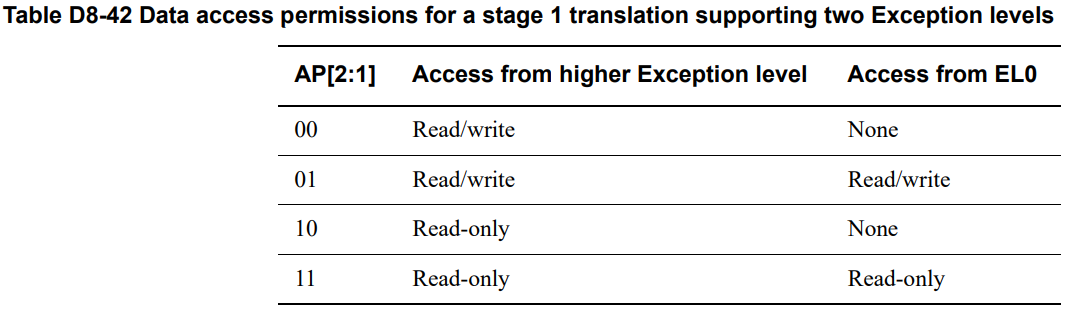
\includegraphics[width=0.7\linewidth]{asserts/AP}
		\caption{ARMv8的定义 AP位}
		\label{fig:ap}
	\end{figure}
	
	\begin{prob} {思考题 6}
		为了简单起见，在 ChCore 实验 Lab1 中没有为内核页表使用细粒度的映射，而是直接沿用了启动时的粗粒度页表，请思考这样做有什么问题。
	\end{prob}

	粗粒度映射是没问题的，只是会造成浪费。毕竟我们专门写了slab机制给内核分配小块内存，内核往往需要使用已知大小的4k以内小块内存。使用大粒度会造成严重浪费。
	
	\begin{prob} {挑战题 7}
		使用前面实现的 \texttt{page\_table.c} 中的函数，在内核启动后的 \texttt{main} 函数中重新配置内核页表，进行细粒度的映射。
	\end{prob}
		我们第一次分配页表是在进入main之前，完成c初始化时。进入main以后，我们很快就会开始初始化buddy和slab。重置页表应该在此操作之前。然而，经过分析，我发现main函数中并没有提供一些物理地址，偏置量，TTBR0等重要宏（这些宏写在了mmu.c中，显然没有为所需实现做准备），且之前的实现完全不足以进行该操作。重置页表的实现是，首先unmap已经分配的页表，然后map新的页表，这需要对块分配的识别。
	
	\begin{prob} {练习题 8}
		完成 \texttt{kernel/arch/aarch64/irq/pgfault.c} 中的 \texttt{do\_page\_fault} 函数中的 \texttt{LAB 2 TODO 5} 部分，将缺页异常转发给 \texttt{handle\_trans\_fault} 函数。
	\end{prob}

	好像就只是转发，
	
	\begin{lstlisting}[style=armasm, language=C]
	ret = handle_trans_fault(current_thread->vmspace, fault_addr);
	\end{lstlisting}

	\begin{prob} {练习题 9}
		完成 \texttt{kernel/mm/vmspace.c} 中的 \texttt{find\_vmr\_for\_va} 函数中的 \texttt{LAB 2 TODO 6} 部分，找到一个虚拟地址在其虚拟地址空间中的 VMR。
	\end{prob}

	该函数可以顾名思义，从虚拟空间获取虚拟地址所在的虚拟段，所以无需看懂整个文件，谢天谢地。课上所述的虚拟空间使用链表组织，这里使用红黑树组织，直接调用红黑树查找即可。

	\begin{lstlisting}[style=armasm, language=C]
	struct rb_node *node = rb_search(&vmspace->vmr_tree, (const void *)addr, cmp_vmr_and_va);
	if (node) {
		return rb_entry(node, struct vmregion, tree_node);
	}
	return NULL;
	\end{lstlisting}

	\begin{prob} {练习题 10}
		完成 \texttt{kernel/mm/pgfault\_handler.c} 中的 \texttt{handle\_trans\_fault} 函数中的 \texttt{LAB 2 TODO 7} 部分（函数内共有 3 处填空，不要遗漏），实现 \texttt{PMO\_SHM} 和 \texttt{PMO\_ANONYM} 的按需物理页分配。你可以阅读代码注释，调用你之前见到过的相关函数来实现功能。
	\end{prob}

	第一处，获得一个页置0。
	
	\begin{lstlisting}[style=armasm, language=C]
	pa = virt_to_phys(get_pages(0));
	memset(phys_to_virt(pa), 0, PAGE_SIZE);
	\end{lstlisting}

	后两处都是分配，调用即可。之前实现的函数没有在头文件给出，但是有一个转接函数。

	\begin{prob} {挑战题 11}
		由于没有磁盘，因此我们采用一部分内存模拟磁盘。内存页是可以换入换出的，请设计一套换页策略（如 LRU 等），并在 \texttt{kernel/mm/pgfault\_handler.c} 中的的适当位置简单实现你的换页方法。
	\end{prob}
	这个实现完全是按照已有策略的工程工作，且还需要另外准备测试函数，故我决定不实现。
	
	\begin{thebibliography}{9}
		\bibitem{arm_architecture_manual}
		ARM. \textit{Arm® Architecture Reference Manual Armv8, for Armv8-A architecture profile}. [Online]. Available: \url{https://developer.arm.com/documentation/ddi0487/latest/}. [Accessed: Nov. 1, 2023].
	\end{thebibliography}
	
	
	\section*{附录}
	See \href{./report_with_code.pdf}{\texttt{report\_with\_code.pdf}}
	
	Grading： \href{./asserts/grading.png}{\texttt{asserts/grading.png}}
%	\begin{lstlisting}[style=armasm, language=C]
%	static struct page *split_chunk(struct phys_mem_pool *pool, int order,
%	struct page *chunk)
%	{
%		/* LAB 2 TODO 1 BEGIN */
%		/*
%		* Hint: Recursively put the buddy of current chunk into
%		* a suitable free list.
%		*/
%		/* BLANK BEGIN */
%		/* A good coding engineer should write handful comments, I was told. */
%		struct page *buddy_chunk;
%		struct free_list *free_list;
%		
%		// BUG_ON(chunk->order < order || chunk->order >= BUDDY_MAX_ORDER); // Could this happen? In case, anyway.
%		
%		/* End of recursive. */
%		if (chunk->order == order) {
%			return chunk;
%		}
%		
%		/* Split the chunk into two smaller chunks. */
%		chunk->order--;
%		buddy_chunk = get_buddy_chunk(pool, chunk); // The buddy chunk is the rest of the input chunk.
%		BUG_ON(buddy_chunk == NULL); // In fact this should never happen if the input chunk is legal.
%		buddy_chunk->order = chunk->order;
%		
%		/* Add the buddy chunk to the free list. */
%		free_list = &pool->free_lists[chunk->order];
%		list_add(&buddy_chunk->node, &free_list->free_list);
%		free_list->nr_free++;
%		
%		/* Recursively split the chunk. */
%		return split_chunk(pool, order, chunk);
%		/* BLANK END */
%		/* LAB 2 TODO 1 END */
%	}
%	\end{lstlisting}
%	\begin{lstlisting}[style=armasm, language=C]	
%	static struct page *merge_chunk(struct phys_mem_pool *pool, struct page *chunk)
%	{
%		/* LAB 2 TODO 1 BEGIN */
%		/*
%		* Hint: Recursively merge current chunk with its buddy
%		* if possible.
%		*/
%		/* BLANK BEGIN */
%		struct page *buddy_chunk;
%		struct list_head *free_list;
%		
%		BUG_ON(chunk->order >= BUDDY_MAX_ORDER); // In case.
%		
%		/* End of recursive. */
%		if (chunk->order == BUDDY_MAX_ORDER - 1){
%			return chunk;
%		}
%		
%		/* Get the buddy chunk of the current chunk. */
%		buddy_chunk = get_buddy_chunk(pool, chunk);
%		/* Must be a legal buddy, but the grading seems to require us to return. */
%		// BUG_ON(buddy_chunk == NULL);
%		
%		/* Check if the buddy chunk is free. */
%		if (buddy_chunk != NULL && !buddy_chunk->allocated && buddy_chunk->order == chunk->order) {
%			/* Update free list. */
%			free_list = &(pool->free_lists[chunk->order].free_list);
%			list_del(&buddy_chunk->node);
%			pool->free_lists[chunk->order].nr_free--;
%			
%			/* Merge ♂ the buddy chunk with the current chunk. */
%			chunk = chunk > buddy_chunk ? buddy_chunk : chunk;
%			chunk->order++;
%			
%			/* Recursively call merge_chunk. */
%			return merge_chunk(pool, chunk);
%		}
%		else {
%			return chunk;    
%		}
%		/* BLANK END */
%		/* LAB 2 TODO 1 END */
%	}
%	\end{lstlisting}
%	\begin{lstlisting}[style=armasm, language=C]	
%	struct page *buddy_get_pages(struct phys_mem_pool *pool, int order)
%	{
%		int cur_order;
%		struct list_head *free_list;
%		struct page *page = NULL;
%		
%		if (unlikely(order >= BUDDY_MAX_ORDER)) {
%			kwarn("ChCore does not support allocating such too large "
%			"contious physical memory\n");
%			return NULL;
%		}
%		
%		lock(&pool->buddy_lock);
%		
%		/* LAB 2 TODO 1 BEGIN */
%		/*
%		* Hint: Find a chunk that satisfies the order requirement
%		* in the free lists, then split it if necessary.
%		*/
%		/* BLANK BEGIN */
%		/* Seek from order. */
%		for (cur_order = order; cur_order < BUDDY_MAX_ORDER; ++cur_order) {
%			free_list = &(pool->free_lists[cur_order].free_list);
%			if (pool->free_lists[cur_order].nr_free) {
%				page = list_entry(free_list->next, struct page, node);
%				list_del(&page->node);
%				pool->free_lists[cur_order].nr_free--;
%				page = split_chunk(pool, order, page);
%				page->allocated = 1;
%				break;
%			}
%		}
%		
%		// BUG_ON(page == NULL); // Failed to allocate memory.
%		
%		
%		/* BLANK END */
%		/* LAB 2 TODO 1 END */
%		out:
%		unlock(&pool->buddy_lock);
%		return page;
%	}
%	\end{lstlisting}
%	\begin{lstlisting}[style=armasm, language=C]
%	void buddy_free_pages(struct phys_mem_pool *pool, struct page *page)
%	{
%		int order;
%		struct list_head *free_list;
%		
%		lock(&pool->buddy_lock);
%		
%		/* LAB 2 TODO 1 BEGIN */
%		/*
%		* Hint: Merge the chunk with its buddy and put it into
%		* a suitable free list.
%		*/
%		/* BLANK BEGIN */
%		/* Deal with freed page first. */
%		page->allocated = 0;
%		page = merge_chunk(pool, page);
%		order = page->order;
%		free_list = &(pool->free_lists[order].free_list);
%		list_add(&page->node, free_list);
%		pool->free_lists[order].nr_free++;
%		/* BLANK END */
%		/* LAB 2 TODO 1 END */
%		
%		unlock(&pool->buddy_lock);
%	}	
%	\end{lstlisting}
%	\begin{lstlisting}[style=armasm, language=C]	
%	static void choose_new_current_slab(struct slab_pointer *pool, int order)
%	{
%		/* LAB 2 TODO 2 BEGIN */
%		/* Hint: Choose a partial slab to be a new current slab. */
%		/* BLANK BEGIN */        
%		struct slab_header *slab;
%		
%		if (list_empty(&pool->partial_slab_list)) {
%			slab = init_slab_cache(order, SIZE_OF_ONE_SLAB);
%			if (slab == NULL) {
%				pool->current_slab = NULL;
%				return;
%			}
%		} else {
%			slab = list_entry(pool->partial_slab_list.next, struct slab_header, node);
%			list_del(&slab->node);
%		}
%		pool->current_slab = slab;
%		/* BLANK END */
%		/* LAB 2 TODO 2 END */
%	}
%	\end{lstlisting}
%	\begin{lstlisting}[style=armasm, language=C]
%	static void *alloc_in_slab_impl(int order)
%	{
%		struct slab_header *current_slab;
%		struct slab_slot_list *free_list;
%		void *next_slot;
%		
%		lock(&slabs_locks[order]);
%		
%		current_slab = slab_pool[order].current_slab;
%		/* When serving the first allocation request. */
%		if (unlikely(current_slab == NULL)) {
%			current_slab = init_slab_cache(order, SIZE_OF_ONE_SLAB);
%			if (current_slab == NULL) {
%				unlock(&slabs_locks[order]);
%				return NULL;
%			}
%			slab_pool[order].current_slab = current_slab;
%		}
%		
%		/* LAB 2 TODO 2 BEGIN */
%		/*
%		* Hint: Find a free slot from the free list of current slab.
%		* If current slab is full, choose a new slab as the current one.
%		*/
%		/* BLANK BEGIN */
%		free_list = current_slab->free_list_head;
%		/* Try new and check. */
%		if (free_list == NULL) {
%			choose_new_current_slab(&slab_pool[order], order);
%			current_slab = slab_pool[order].current_slab;
%			if (current_slab == NULL) {
%				unlock(&slabs_locks[order]); // Don't forget this.
%				return NULL;
%			}
%			free_list = current_slab->free_list_head;
%		}
%		
%		next_slot = free_list->next_free;
%		current_slab->free_list_head = next_slot;
%		current_slab->current_free_cnt--;
%		/* BLANK END */
%		/* LAB 2 TODO 2 END */
%		
%		unlock(&slabs_locks[order]);
%		
%		return (void *)free_list;
%	}	
%	\end{lstlisting}
%	\begin{lstlisting}[style=armasm, language=C]	
%	void free_in_slab(void *addr)
%	{
%		struct page *page;
%		struct slab_header *slab;
%		struct slab_slot_list *slot;
%		int order;
%		
%		slot = (struct slab_slot_list *)addr;
%		page = virt_to_page(addr);
%		if (!page) {
%			kdebug("invalid page in %s", __func__);
%			return;
%		}
%		
%		
%		slab = page->slab;
%		order = slab->order;
%		lock(&slabs_locks[order]);
%		
%		try_insert_full_slab_to_partial(slab);
%		
%		#if ENABLE_DETECTING_DOUBLE_FREE_IN_SLAB == ON
%		/*
%		* SLAB double free detection: check whether the slot to free is
%		* already in the free list.
%		*/
%		if (check_slot_is_free(slab, slot) == 1) {
%			kinfo("SLAB: double free detected. Address is %p\n",
%			(unsigned long)slot);
%			BUG_ON(1);
%		}
%		#endif
%		
%		/* LAB 2 TODO 2 BEGIN */
%		/*
%		* Hint: Free an allocated slot and put it back to the free list.
%		*/
%		/* BLANK BEGIN */
%		slot->next_free = slab->free_list_head;
%		slab->free_list_head = (void *)slot;
%		slab->current_free_cnt++;
%		/* BLANK END */
%		/* LAB 2 TODO 2 END */
%		
%		try_return_slab_to_buddy(slab, order);
%		
%		unlock(&slabs_locks[order]);
%	}
%	\end{lstlisting}
%	\begin{lstlisting}[style=armasm, language=C]	
%	void *_kmalloc(size_t size, bool is_record, size_t *real_size)
%	{
%		void *addr;
%		int order;
%		
%		if (unlikely(size == 0))
%		return ZERO_SIZE_PTR;
%		
%		if (size <= SLAB_MAX_SIZE) {
%			/* LAB 2 TODO 3 BEGIN */
%			/* Step 1: Allocate in slab for small requests. */
%			/* BLANK BEGIN */
%			addr = alloc_in_slab(size, real_size);
%			/* BLANK END */
%			#if ENABLE_MEMORY_USAGE_COLLECTING == ON
%			if(is_record && collecting_switch) {
%				record_mem_usage(*real_size, addr);
%			}
%			#endif
%		} else {
%			/* Step 2: Allocate in buddy for large requests. */
%			/* BLANK BEGIN */
%			order = size_to_page_order(size);
%			addr = get_pages(order);
%			/* BLANK END */
%			/* LAB 2 TODO 3 END */
%		}
%		
%		BUG_ON(!addr);
%		return addr;
%	}
%	\end{lstlisting}
%	\begin{lstlisting}[style=armasm, language=C]	
%	int query_in_pgtbl(void *pgtbl, vaddr_t va, paddr_t *pa, pte_t **entry)
%	{
%		/* LAB 2 TODO 4 BEGIN */
%		/*
%		* Hint: Walk through each level of page table using `get_next_ptp`,
%		* return the pa and pte until a L0/L1 block or page, return
%		* `-ENOMAPPING` if the va is not mapped.
%		*/
%		/* BLANK BEGIN */
%		ptp_t *l0_ptp, *l1_ptp, *l2_ptp, *l3_ptp, *vp;
%		pte_t *pte;
%		int ret;
%		
%		/* L0 page table */ 
%		l0_ptp = (ptp_t *)pgtbl;
%		ret = get_next_ptp(l0_ptp, L0, va, &l1_ptp, &pte, false, NULL);
%		if (ret < 0) {
%			return ret;
%		}
%		
%		/* L1 page table */ 
%		ret = get_next_ptp(l1_ptp, L1, va, &l2_ptp, &pte, false, NULL);
%		if (ret < 0) {
%			return ret;
%		}
%		else if (ret == BLOCK_PTP) {
%			if (entry != NULL) {
%				*entry = pte;
%			}
%			*pa = virt_to_phys(l2_ptp) + GET_VA_OFFSET_L1(va);
%			return 0;
%		}
%		
%		
%		/* L2 page table */
%		ret = get_next_ptp(l2_ptp, L2, va, &l3_ptp, &pte, false, NULL);
%		if (ret < 0) {
%			return ret;
%		}        
%		else if (ret == BLOCK_PTP) {
%			if (entry != NULL) {
%				*entry = pte;
%			}
%			*pa = virt_to_phys(l3_ptp) + GET_VA_OFFSET_L2(va);
%			return 0;
%		}
%		
%		/* L3 page table */ 
%		ret = get_next_ptp(l3_ptp, L3, va, &vp, &pte, false, NULL);
%		if (ret < 0) {
%			return ret;
%		}
%		if (entry != NULL) {
%			*entry = pte;
%		}
%		*pa = virt_to_phys(vp) + GET_VA_OFFSET_L3(va);
%		/* LAB 2 TODO 4 END */
%		return 0;
%	}
%	\end{lstlisting}
%	\begin{lstlisting}[style=armasm, language=C]
%	static int map_range_in_pgtbl_common(void *pgtbl, vaddr_t va, paddr_t pa, size_t len,
%	vmr_prop_t flags, int kind, long *rss)
%	{
%		/* LAB 2 TODO 4 BEGIN */
%		/*
%		* Hint: Walk through each level of page table using `get_next_ptp`,
%		* create new page table page if necessary, fill in the final level
%		* pte with the help of `set_pte_flags`. Iterate until all pages are
%		* mapped.
%		* Since we are adding new mappings, there is no need to flush TLBs.
%		* Return 0 on success.
%		*/
%		/* BLANK BEGIN */
%		ptp_t *l0_ptp, *l1_ptp, *l2_ptp, *l3_ptp;
%		pte_t *pte;
%		int ret;
%		
%		l0_ptp = (ptp_t *)pgtbl;
%		size_t allocated_size = 0;
%		vaddr_t cur_va = va;
%		paddr_t cur_pa = pa;
%		
%		while (allocated_size < len) {
%			
%			/* Find the L3. */
%			ret = get_next_ptp(l0_ptp, L0, cur_va, &l1_ptp, &pte, true, rss);
%			if (ret < 0) {
%				return ret;
%			}
%			
%			ret = get_next_ptp(l1_ptp, L1, cur_va, &l2_ptp, &pte, true, rss);
%			if (ret < 0) {
%				return ret;
%			}
%			
%			ret = get_next_ptp(l2_ptp, L2, cur_va, &l3_ptp, &pte, true, rss);
%			if (ret < 0) {
%				return ret;
%			}
%			
%			/* Mapping. */
%			for (int ent_i = GET_L3_INDEX(cur_va); ent_i < PTP_ENTRIES; ++ent_i) {
%				pte_t t_pte;
%				
%				t_pte.pte = 0;
%				t_pte.l3_page.is_valid = 1;
%				t_pte.l3_page.is_page = 1;
%				t_pte.l3_page.pfn = cur_pa >> PAGE_SHIFT;
%				set_pte_flags(&t_pte, flags, USER_PTE);
%				l3_ptp->ent[ent_i].pte = t_pte.pte;
%				
%				/* A new page allocated in L3. */
%				allocated_size += PAGE_SIZE;
%				// *rss += PAGE_SIZE; // ??????wtf
%				cur_va += PAGE_SIZE;
%				cur_pa += PAGE_SIZE;
%				if (allocated_size >= len) {
%					break;
%				}
%			}
%		}
%		/* BLANK END */
%		/* LAB 2 TODO 4 END */
%		return 0;
%	}	
%	\end{lstlisting}
%	\begin{lstlisting}[style=armasm, language=C]	
%	int unmap_range_in_pgtbl(void *pgtbl, vaddr_t va, size_t len, long *rss)
%	{
%		/* LAB 2 TODO 4 BEGIN */
%		/*
%		* Hint: Walk through each level of page table using `get_next_ptp`,
%		* mark the final level pte as invalid. Iterate until all pages are
%		* unmapped.
%		* You don't need to flush tlb here since tlb is now flushed after
%		* this function is called.
%		* Return 0 on success.
%		*/
%		/* BLANK BEGIN */
%		ptp_t *l0_ptp, *l1_ptp, *l2_ptp, *l3_ptp;
%		pte_t *pte;
%		int ret;
%		
%		l0_ptp = (ptp_t *)pgtbl;
%		size_t unmapped_size = 0;
%		vaddr_t cur_va = va;
%		
%		while (unmapped_size < len) {
%			
%			/* Find the L3. */
%			ret = get_next_ptp(l0_ptp, L0, cur_va, &l1_ptp, &pte, false, rss);
%			if (ret < 0) {
%				return ret;
%			}
%			
%			ret = get_next_ptp(l1_ptp, L1, cur_va, &l2_ptp, &pte, false, rss);
%			if (ret < 0) {
%				return ret;
%			}
%			
%			ret = get_next_ptp(l2_ptp, L2, cur_va, &l3_ptp, &pte, false, rss);
%			if (ret < 0) {
%				return ret;
%			}
%			
%			/* Freeing. */
%			for (int ent_i = GET_L3_INDEX(cur_va); ent_i < PTP_ENTRIES; ++ent_i) {
%				l3_ptp->ent[ent_i].pte = PTE_DESCRIPTOR_INVALID;
%				
%				cur_va += PAGE_SIZE;
%				unmapped_size += PAGE_SIZE;
%				if (unmapped_size >= len) {
%					break;
%				}
%			}
%		}
%		/* BLANK END */
%		/* LAB 2 TODO 4 END */
%		
%		dsb(ishst);
%		isb();
%		
%		return 0;
%	}
%	\end{lstlisting}
\end{document}